
%% add 'handout' option for handouts, and pgfpages for 2-on-1
\documentclass[smaller,compress]{beamer}   
%\usepackage{pgfpages}
%\pgfpagesuselayout{2 on 1}[letterpaper,border shrink=5mm]
%\pgfpagesuselayout{4 on 1}[letterpaper,border shrink=5mm]
%\pgfpagesuselayout{2 on 1}[a4,border shrink=5mm]


\mode<presentation>
{
  %\usetheme[secheader]{Madrid} % nice (once my coloroverrides are sorted out)
  %\usetheme{AnnArbor}	% nice!	
  %\usetheme{Malmoe}	% nice!	
  \usetheme{Warsaw}	% nice!	

  %\usetheme[secheader]{Boadilla} % ok
  %\usecolortheme{whale}
  %\usecolortheme{orchid}
}

% Delete this, if you do not want the table of contents to pop up at
% the beginning of each subsection (or section)
% edd: Does not work in handout mode, and we have too many section/subsections
%\AtBeginSection[]{%
%  \begin{frame}<beamer>%
%    %\tiny
%    \frametitle{Outline}%
%    \tableofcontents[currentsection]%
%  \end{frame}
%}


% If you wish to uncover everything in a step-wise fashion, uncomment the following command: 
%\beamerdefaultoverlayspecification{<+->}

\newcommand{\MedSkip}{\medskip \par} % add \pause if desired 
\newcommand{\SmallSkip}{\smallskip} % add \pause if desired 

\usepackage[english]{babel}   	% or whatever
\usepackage[latin1]{inputenc}	% or whatever
\usepackage{times}
\usepackage[T1]{fontenc}	% Or whatever. Note that the encoding and the 
				% font should match. If T1 does not look
                                % nice, try deleting the line with the fontenc.
%\usepackage{highlight}

\usepackage{listings}
\lstset{ %
  language=R,                   % choose the language of the code
  basicstyle=\scriptsize,       % the size of the fonts that are used for the code
  numbers=left,                 % where to put the line-numbers
  numberstyle=\tiny,            % the size of the fonts that are used for the line-numbers
  stepnumber=1,                 % the step between two line-numbers. If it's 1 each line will be numbered
  numbersep=5pt,                % how far the line-numbers are from the code
  backgroundcolor=\color{white},% choose the background color. You must add \usepackage{color}
  showspaces=false,             % show spaces adding particular underscores
  showstringspaces=false,       % underline spaces within strings
  showtabs=false,               % show tabs within strings adding particular underscores
  frame=single,                 % adds a frame around the code
  tabsize=2,                    % sets default tabsize to 2 spaces
  captionpos=b,                 % sets the caption-position to bottom
  breaklines=true,              % sets automatic line breaking
  breakatwhitespace=false,      % sets if automatic breaks should only happen at whitespace
  escapeinside={\%*}{*)}        % if you want to add a comment within your code
}

\hypersetup{                  		% beamer colors taken from elsewhere
  hyperindex,%				% works with the beetle colour scheme
  colorlinks,%
  linktocpage,%
  plainpages=true,%
  linkcolor=myOrange,%
  citecolor=myDarkGrey,%
  urlcolor=myDarkBlue,%
  pdfstartview=Fit,%
  pdfview={XYZ null null null}%
}
%\hypersetup{                  		% beamer colors taken from elsewhere
%  hyperindex,%				% works with the beetle colour scheme
%  colorlinks%
%  linktocpage,%
%  plainpages=false,%
%  linkcolor=eddBlue,%
%  citecolor=eddDarkGrey,%
%  urlcolor=eddDarkBlue,%
%  pdfstartview=Fit,%
%  pdfview={XYZ null null null}%
%}

\RequirePackage{color}
\definecolor{Red}{rgb}{0.7,0,0}
\definecolor{myOrange}{rgb}{0.8,0.5,0.0}
\definecolor{myBlue}{rgb}{0.0,0.0,0.4}
\definecolor{myDarkBlue}{rgb}{0.1,0.1,0.4}
\definecolor{myDarkGrey}{rgb}{0.15,0.15,0.15}
% Doug's
\definecolor{Sinput}{rgb}{0,0,0.56}
\definecolor{Scode}{rgb}{0,0,0.56}
\definecolor{Soutput}{rgb}{0.56,0,0}
% 
\definecolor{Cmdinput}{rgb}{0,0,0.44}
\definecolor{Cmdoutput}{rgb}{0.44,0,0}
\definecolor{Cppinput}{rgb}{0.15,0.15,0.15}

%% from Doug, but mod'ed \R to use hyperref
\RequirePackage{fancyvrb}
\RequirePackage{xspace}
\RequirePackage{paralist}
\newenvironment{Schunk}{\par\begin{minipage}{\textwidth}}{\end{minipage}}
\DefineVerbatimEnvironment{Sinput}{Verbatim}{formatcom={\color{Sinput}},fontsize=\small}
\DefineVerbatimEnvironment{Soutput}{Verbatim}{formatcom={\color{Soutput}},fontsize=\footnotesize}
\DefineVerbatimEnvironment{Scode}{Verbatim}{formatcom={\color{Scode}},fontsize=\small}
\DefineVerbatimEnvironment{Cmdinput}{Verbatim}{formatcom={\color{Cmdinput}},fontsize=\small}
\DefineVerbatimEnvironment{Cmdoutput}{Verbatim}{formatcom={\color{Cmdoutput}},fontsize=\footnotesize}
\DefineVerbatimEnvironment{Cppinput}{Verbatim}{formatcom={\color{Cppinput}},fontsize=\small}

% -- not \small 
\newcommand{\smallcode}[1]{{\color{Sinput}\small\texttt{#1}}}
\newcommand{\code}[1]{{\color{Sinput}\texttt{#1}}}
\newcommand{\Emph}[1]{\emph{\color{Scode}#1}}   
%\newcommand{\R}{\href{http://www.r-project.org}{\Emph{R}\xspace}}   %% ? sing \emph upsets beamer inside \href
\newcommand{\R}{\href{http://www.r-project.org}{\textsf{R}\xspace}}
\newcommand{\Rns}{\href{http://www.r-project.org}{\textsf{R}}}

% two old defintions
%\newcommand{\code}[1]{\texttt{#1}}
\newcommand{\screenshot}[1]{\centerline{\includegraphics[height=7.8cm,transparent]{#1}}}  % 7.8in


% If you have a file called "university-logo-filename.xxx", where xxx
% is a graphic format that can be processed by latex or pdflatex,
% resp., then you can add a logo as follows:
% NB transparent in Adobe but not in kpdf
\pgfdeclareimage[height=0.6cm]{useR-logo}{figures/useR}
\logo{\pgfuseimage{useR-logo}}


%%% Local Variables: 
%%% mode: latex
%%% TeX-master: "introhighperfR"
%%% End: 
  %% has all definitions etc

%\title[cran2deb: Automated CRAN to Debian packages generation]{cran2deb: A
%  system to automatically provide 1700+ CRAN packages as Debian binaries} 
\title[cran2deb: CRAN to Debian packages]{cran2deb:  A fully automated CRAN to \\
  Debian package generation system} 
\subtitle{\textsl{UseR! 2009 Presentation}}
\subject{UseR! 2009 Presentation}
\author[Charles Blundell \and Dirk Eddelbuettel]{Charles Blundell\inst{1} \and Dirk Eddelbuettel\inst{2}}
\institute[Gatsby \and Debian]{\inst{1}Gatsby Computational Neuroscience Unit
  \\ University College London, UK \and \inst{2}Debian and R Projects \\ Chicago,
IL, USA}
%\date[UseR! 2009]{Presentation at UseR! 2009 \\ Rennnes, France \\ July 2009}
\date[UseR! 2009 Presentation]{Universit\'{e} Rennes II, Agrocampus Ouest \\ Laboratoire de
  Math\'{e}matiques Appliqu\'{e}es \\ 8-10 July 2009}


\begin{document}

\begin{frame}
  \titlepage
\end{frame}

\begin{frame}
  \frametitle{Overview}
  \tableofcontents
\end{frame}

\section[Why]{Why: Background and Motivation}
\begin{frame}
  \frametitle{About R -- and its repositories}
  \framesubtitle{An open statistical language / environment -- with lots of
    excellent code contributions}

  A few key facts that are non-controversial at a \textsl{useR!} conference:
  \begin{itemize} 
  \item \R\ is now a standard for statistical applications and research
  \item \textit{``Success has many fathers''}: several key drivers can
    be identified as to why \R\ has done so well 
  \item We would like to stress \textsl{repositories} and available packages here:
    CRAN, as well as BioConductor and Omegahat.
  \item CRAN has been one of the drivers: an open yet rigorously QA'ed
    repository which has experienced tremendous growth
  \end{itemize}
\end{frame}

\begin{frame}
  \frametitle{CRAN Packages} %% NB Or shall we merge this with the preceding slide?
  \framesubtitle{Exponential Growth}

  \begin{columns}
    \begin{column}{3in}
      \begin{figure}
        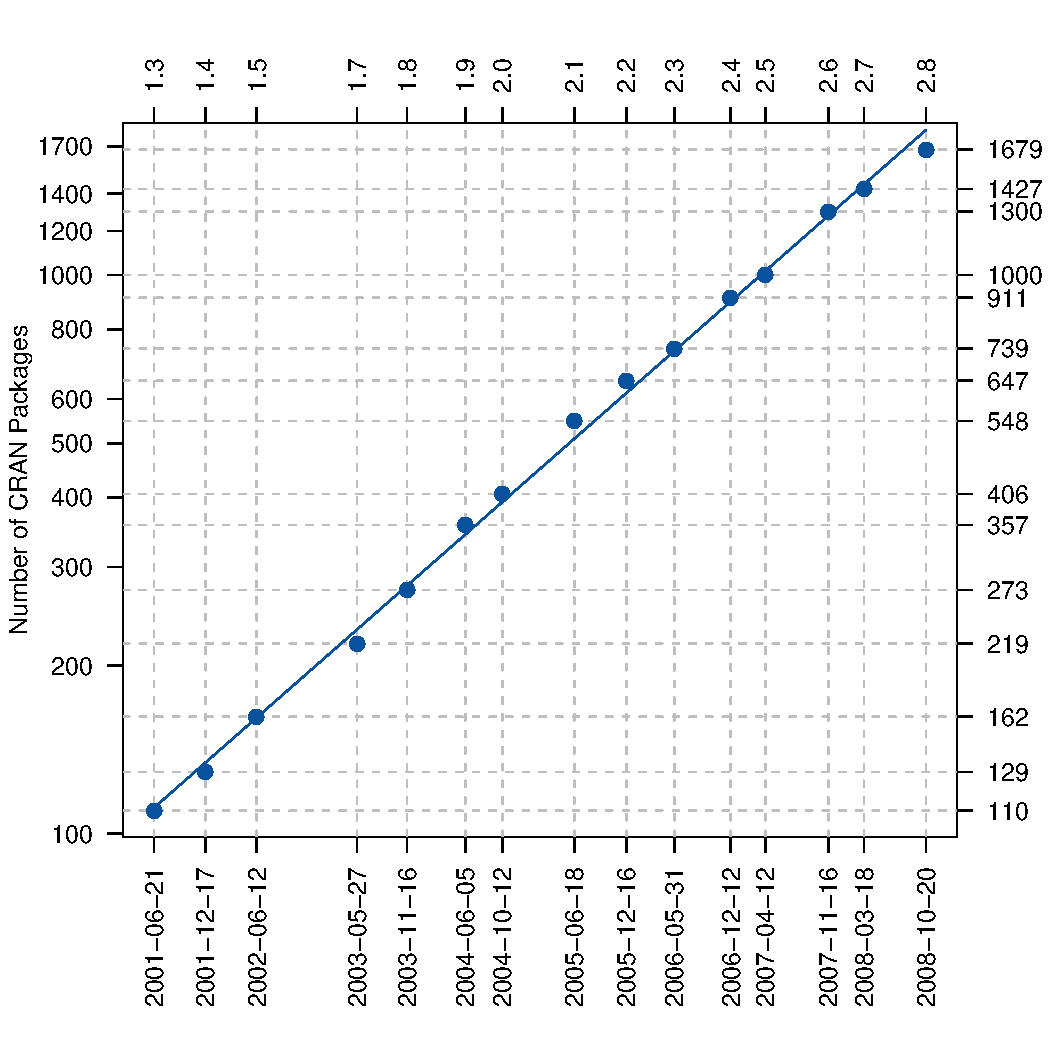
\includegraphics[height=6cm,transparent]{figures/Packages}

        \begin{scriptsize}
          Source: Fox (2008, 2009), our calculations
        \end{scriptsize}
      \end{figure}
    \end{column}
    \begin{column}{2in}
      \begin{itemize} 
        \item CRAN archive network growing by 40\% p.a., now at around 1750 packages

        \item John Fox provided this chart in an invited lecture at the last
        \emph{useR!} meetings.
      \end{itemize}
    \end{column}
    \begin{column}{0.25in}
      \phantom{XX}
    \end{column}
  \end{columns}  
\end{frame}

\begin{frame}
  \frametitle{Debian and Ubuntu} % NB Maybe skip this slide?
  \framesubtitle{Open Linux distributions}

  A few key points:
  \begin{itemize} 
  \item Debian is \textsl{the} community-driven Linux distribution where
    numerous volunteers provide over twenty-thousand packages for around
    a dozen architectures.
  \item Packages and package management ``just work'': with arguably the most
    advanced and robust package management system, and a tremendous
    build and test infrastructure.
  \item Ubuntu has taken Debian, added a fair amount of spit and polish, as
    well as regular bi-annual releases, and has rapidly gained mind- and
    well as market-share as the Linux distribution to beat.
  \item We also note that the CRAN backend is implemented on Debian.
  \end{itemize}
\end{frame}

\begin{frame}
  \frametitle{Why build Debian R packages?}
  \framesubtitle{Combining R and Debian}
  Bates, Eddelbuettel and Gebhard (UseR! 2004) listed a number of reason
  that still hold:
  \begin{itemize} 
  \item \textbf{Dependencies} are resolved automatically: \textsl{it just
      works}
  \item \textbf{Convenience} of installing binary packages via
    \texttt{apt-get} %is
    %easier than building from source
  \item \textbf{Quality control} as build daemons, automated rebuilds,
    porting, ... all ensure that everything is pretty much buildable all the
    time
  \item \textbf{Scalability} as building one binary package and scripting
    installation on a cluster beats doing lots of manual installations
  \item \textbf{Common platform} as Debian forms the base for Ubuntu and
    several other derivative or single-focus distributions
  \item \textbf{Different architectures} ranging from small arm or MIPS based
    systems to amd64, sparc64, hppa or even s390 mainframes
  \item \textbf{Audience} given the reach of Debian and Ubuntu, large number
    of users can be reached with little effort
  \end{itemize}

\end{frame}

%\section{What is behind it?}
%\begin{frame}
%  \frametitle{So what is a Debian package?} % NB Maybe skip this?
%  \framesubtitle{And how do I build it?}
%
%  Building a Debian package is similar to using \texttt{R
%    CMD binary} etc:
%  \begin{itemize} 
%  \item Reads meta-information is read from the files in the debian/ directory
%    \begin{itemize} 
%    \item debian/control (similar to R's DESCRIPTION) lists names,
%      maintainers, build- and run-time dependencies
%    \item debian/copyright lists all author, license holders and copyright
%      statements 
%    \item debian/changelog provides current and past version numbers with a
%      list of  all changes in chronological fashion
%    \item debian/rules is a Makefile containing all steps to configure,
%      build, install, package-create and clean
%    \end{itemize}
%  \item Employs a number of external tools scripts and tools, can be used
%    interactively or in batch mode in chroot'ed 'clean rooms'
%  \end{itemize}
%\end{frame}


\section[How]{How: Key aspects of the approach and implementation}
\begin{frame}
  \frametitle{Comparing two approaches}
  \framesubtitle{What have we learned?}

  Eddelbuettel, Vernazobres, Gebhard and M\"{o}ller (UseR 2007) presented a first
  approach.

  \MedSkip

  \begin{columns}
    \begin{column}{2in}
      \textsl{Then}
      \begin{itemize}
      \item Top-down approach 
      \item Monolithic and large Perl program 
      \item Meta-information encode directly as Perl hashes in program
      \item Re-implementing chunks of what \R does in parsing archives
      \item Not very robust
      \end{itemize}
    \end{column}      

    \begin{column}{2in}
      \textsl{Now}
      \begin{itemize}
      \item Bottom-up approach
      \item Collection of \R and shell scripts, also lots of SQL
      \item Re-using \R internal infrastructure as much as possible
      \item Influenced by %Eddelbuettel's
        \href{http://dirk.eddelbuettel.com/cranberries/}{CRANberries} and its
        200 lines of \R code to monitor and summarize CRAN changes
      \end{itemize}
    \end{column}      
  \end{columns}
\end{frame}

\begin{frame}
  \frametitle{Technology Overview: Big Picture}
  \framesubtitle{Key components}

  cran2deb is implemented as a collection of small tools:
  \begin{itemize}
  \item cran2deb is just a wrapper script calling out to twenty-one other
    'worker' scripts implementing the twenty-one basic high-level commands
    \begin{itemize}
    \item 'worker' scripts are written in \R (for littler), Korn/Bash shell,
      and in the Plan9 shell rc
      \item all these scripts are small: the largest is 4 kb and only seven
        are larger than 1 kb
      \item this is recursive: 'help' is one of these scripts scanning for
        doc-strings in the other scripts
    \end{itemize}
  \item cran2deb is also an R package that is being called by some of the R
    scripts; the R package has just over 1500 lines of code, and it calls out
    to R functionality from package utils and tools.
  \end{itemize}
\end{frame}  

\begin{frame}
  \frametitle{Technology Overview} 
  \framesubtitle{A walk through}

  cran2deb:
  \begin{itemize}
  \item pulls meta-data updates from CRAN daily via R's available.packages
  \item detects new or changed packages and gets building each one:
    \begin{itemize}
      \item Map declared R dependencies onto cran2deb packages
      \item Map free-form SystemRequirements onto Debian packages
        \begin{itemize}
          \item Rules for this shared among packages---many packages ``just work''.
        \end{itemize}
      \item Add any undeclared dependencies that we found were needed (applies to just 36 packages).
      \item Build each package in its own isolated, clean, fresh, up to date Debian environment via pbuilder.
        \begin{itemize}
          \item Looks like a fresh install of Debian; ensures correctness of dependencies.
          \item Check package quality via Debian's lintian.
        \end{itemize}
    \end{itemize}
  \end{itemize}
  RSQLite backend for cran2deb state: everything from package meta-information, blacklist of bad packages, to build logs.
\end{frame}  

\begin{frame}
  \frametitle{Technology Overview} 
  \framesubtitle{Continued}

  Re-use, re-duce, re-cycle:

  \begin{itemize}
  \item \R's infrastructure is used for obtaining the \R view of the world:
    what packages and where, first approximation to dependencies.
  \item All this makes use of Debian build infrastructure, notably the
    pbuilder chroot environment and the package management system
  \item cran2deb sets the build environment up by invoking the proper Debian
    scripts 
  \item the `production line' of packages is fully automated via cron and report status
    summaries by email
  \item per-package patches are allowed (currently eleven packages have
    mostly trivial patches)
  \item source code is available via the r-forge subversion repository and archive
  \end{itemize}

\end{frame}

\section[Status]{Status: Where are we now?}

\begin{frame}
  \frametitle{Building 1700+ package}
  \framesubtitle{Summary from a package views}

  It's easy: basically \textsl{everything} builds and is available as a
  Debian package (complete with full dependencies) --- apart from:

  \begin{itemize}
  \item 17 packages that are \textsl{not free enough}:\footnote{Generally these
do not allow commercial use, modification and/or distribution with the
exception of ConvCalendar which gives no modification or distribution rights.}
    mclust, mclust02, ConvCalendar, SDDA, conf.design, isa2, optmatch,
    rankreg, realized, rngwell19937, tnet, spatialkernel, Bhat, PTAk,
    PredictiveRegression, RLadyBug, mapproj 
  \item 1 package that is obsolete: xgobi
  \item 2 package that break building packages via cran2deb:\footnote{It
      takes down the cronjob; we are stumped as to why.} dprep, EngrExpt
  \item 1 package that is not built for 'other' reasons:\footnote{It contains
      binary code.} sabreR
  \end{itemize}
\end{frame}

\begin{frame}
  \frametitle{Building 1700+ package}
  \framesubtitle{Continued}

  \begin{itemize}
  \item 47 packages that have \textsl{unsatisfied
      dependencies}:\footnote{Some require other commercial software, some
      require software we classified\newline as non-free, some require BioConductor packages.}
    ROracle, Rlsf, Rsge, CarbonEL, VhayuR, gputools, klaR, wgaim, svGUI,
    RScaLAPACK, caMassClass, Rcplex, ADaCGH, DAAGbio, GFMaps, GOSim,
    Metabonomic, classGraph, gcExplorer, logilasso, pcalg, celsius, multtest,
    hopach, GExMap, LMGene, PCS, SubpathwayMiner, gene2pathway, PhViD,
    SNPMaP, qdg, lsa, mpm, sisus, metaMA, clustTool, clustvarsel,
    SpectralGEM, bayesCGH, crosshybDetector  
  \item 7 package that (as of end of June) fails for unclassified reasons:
    IDPmisc, Rsymphony, SuppDists, aroma.apd, aroma.core, cmprskContin, mvgraph
  \end{itemize}

  \MedSkip
  \textsl{But everything else}---currently 1768 packages---builds and is
  available via \texttt{apt-get} and other package management frontends!
\end{frame}  

\begin{frame}
  \frametitle{Status and credits}
  \framesubtitle{Ready for wider deployment and testing}

  Who do we owe, and where is it at: 

  \begin{itemize}
  \item The ground-work was provided during Google Summer of Code (GSoC) 2008 under the
    umbrella of the Debian project. We thank Google for the GSoC support.
  \item Currently we are using a (small) Xen-instance on a server at WU Wien to host
    two Debian pbuilder chroots and an archive. We thank WU Wien/CRAN for
    hosting and cpu cycles.
  \item 1700+ packages for i386 and amd64 on Debian testing
  \item In daily use for the last few weeks!
  \end{itemize}

  \MedSkip
  So just add one of these URLs:\newline
  i386 \phantom{xx} : { \SmallSkip \scriptsize
    \texttt{deb http://xmcorsairs.wu.ac.at/cran2deb/debian-i386 testing/}
  } \newline
  amd64 : { \SmallSkip \scriptsize
    \texttt{deb http://xmcorsairs.wu.ac.at/cran2deb/debian-amd64 testing/}
  }

\end{frame}

\section{Open Issues}
\begin{frame}
  \frametitle{Question to be addressed}
  \framesubtitle{These may not be showstoppers}

  Things that still need to be sorted out:
  \begin{itemize}
  \item What can or cannot be (re-)distributed by CRAN and its mirrors?
  \item What can or cannot be used by all users?
  \item Remaining external dependencies: 
    \begin{itemize}
      \item BioConductor is the single largest source: BioBase, RGraphviz, etc
      \item Other external libraries or tools not in Debian 
      \item Commercial external dependencies: SGE, LSF, Oracle, Vhayu
    \end{itemize}
  \item Builds for other architectures?
  \item Builds for other Debian flavours such as Ubuntu?
  \end{itemize}
\end{frame}

\end{document}

%%% Local Variables: 
%%% mode: latex
%%% TeX-master: t
%%% End: 
